

\documentclass[10pt]{article}
\usepackage{hyperref}
\usepackage{amsmath}
% amssymb package, useful for mathematical symbols
\usepackage{amssymb}
\usepackage[hangul]{kotex}
\usepackage{url}
\usepackage{tabularx}
\usepackage{array}
\usepackage{rotating}
\usepackage{graphicx}
\usepackage[caption = false]{subfig}
\topmargin 0.0cm
\oddsidemargin 0.5cm
\evensidemargin 0.5cm
\textwidth 16cm 
\textheight 21cm

\newcommand\abs[1]{\left|#1\right|}

\title{\textbf{딥러닝(Deep Learning)의 역사와 현재, 그리고 보건학으로의 적용}}
\author{
        \textbf{김진섭}            
}
\date{\today}


\begin{document}
\maketitle

\begin{abstract}
최근 유행하는 기계학습(Machine Learning) 방법인 딥러닝(Deep Learning)에 대해 알아보고 보건학으로의 적용 가능성에 대해 말해본다. 
\end{abstract}

\section{서론} %필요성 
\noindent 기계학습(Machine Learning)은 컴퓨터가 스스로 학습하여 예측모형을 개발하는 인공지능의 한 분야이며,  딥러닝(Deep Learning)은 인간의 신경망의 원리를 이용한 심층신경망(Deep Neural Network)이론을 이용한 기계학습방법이다. 딥러닝 기술은 이미 구글, 페이스북, 아마존 등 글로벌 IT기업들에서 광범위하게 이용되고 있는 기술이며 특히, 패턴인식이나 사진, 음성 등의 인식, 기계번역 등의 자연언어처리(Natural Language Processing)에 좋은 성능을 발휘하는 것으로 알려져 있는데,  MIT가 2013년을 빛낼 10대 혁신기술 중 하나로 선정하고 가트너(Gartner, Inc.)가 2014 세계 IT 시장 10대 주요 예측기술로 언급하는 등 최근 가장 뜨거운 이슈가 되고 있다\cite{mitnews,gartnernews}. 딥러닝이 기존의 통계학이나 다른 기계학습 방법과 다른 큰 차이점은 인간의 뇌를 기초로하여 설계되었다는 점이다. 인간은 컴퓨터가 아주 짧은 시간에 할 수 있는 계산도 쉽게 해낼 수 없는 반면, 컴퓨터는 인간이 쉽게 인지하는 사진이나 음성을 해석하지 못하는데 이는 인간의 뇌가 엄청난 수의 뉴런과 시냅스의 \textbf{병렬연결}로 이루어져 있기 때문이다. 각각의 뉴런은 기능이 보잘것 없지만 수많은 뉴런들이 복잡하게 연결되어 병렬연산을 수행함으로서 컴퓨터가 하지 못하는 음성, 영상인식을 수월하게 할 수 있는 것이며 딥러닝은 이 수많은 뉴런과 시냅스의 병렬연산을 컴퓨터로 재현하는 방법인 것이다. 이것이 글로벌 IT기업들이 딥러닝을 주목하는 이유일 것이다. 이에 본 글에서는 인공신경망 이론의 역사부터 현재 상황까지를 간략히 리뷰해 볼 것이며 이 방법이 공중보건을 향상시키는데 어떻게 이용될 수 있을 것인지 생각해 보도록 하겠다. 


\section{딥러닝의 역사}
딥러닝의 역사는 크게 3시기로 나뉘어지는데 1세대는 최초의 인경신공망인 퍼셉트론(Perceptron), 2세대는 다층(Multilayer) 퍼셉트론, 그리고 현재의 딥러닝을 3세대라고 할 수 있을 것이다. 


\subsection{1세대: Perceptron}
인공신경망(Neural Network)의 기원은 1958년에 Rosenblatt가 제안한 퍼셉트론이 시작이라 할 수 있다\cite{rosenblatt1958perceptron}. $n$개의 input과 1개의 output에 대하여 각각의 input의 weight를 $w_i$라 한 후 퍼셉트론을 수식으로 나타내면 다음과 같다(그림 \ref{perceptron1})\cite{perceptronfig}.

\begin{align}
y=\varphi(\sum_{i=1}^n w_ix_i+b)
\end{align}
($b$: bias, $\varphi$: activation function(e.g: logistic or $tanh$)

\begin{figure}[!ht]
\centering
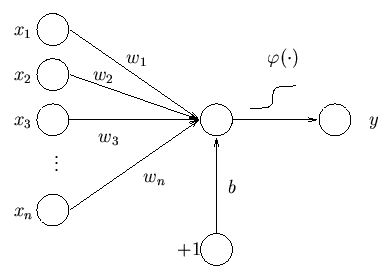
\includegraphics[width=3in]{/home/secondmath/Dropbox/GSPH/topic_review/DNN/perceptron.png}
\caption{\bf {Concept of Perceptron}}
\label{perceptron1}
\end{figure}

즉 $n$개의 input의 선형결합(Linear Combination)에 Activation 함수를 적용하여 0$\sim$1 사이의 확률값으로 $y$값을 제공하는 것이며, 확률값으로 받은 후에는 편의에 따라 0를 기준으로 event냐 아니냐(1 VS -1)를 판단한다. \\

이것이 인공신경망 모형의 시작이다. 허나 이 모형은 아주 간단한 XOR problem마저 학습하지 못하는 등, 심각한 문제가 있는데(그림 \ref{perceptron2}) 이 때문에 한동안 발전없이 포류되게 된다\cite{perceptroncant}.


\begin{figure}[!ht]
\centering
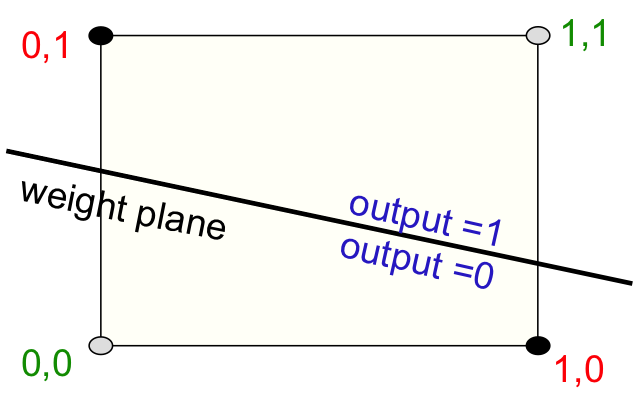
\includegraphics[width=3in]{/home/secondmath/Dropbox/GSPH/topic_review/DNN/notperceptron.png}
\caption{\bf {XOR problem in  Perceptron}}
\label{perceptron2}
\end{figure}

\subsection{2세대: Multilayer Perceptron}
XOR등 간단한 것도 학습하지 못하는 퍼셉트론의 단점을 해결하기 위한 방법은 의외로 단순하였는데 Input layer와 output layer사이에 하나 이상의 hidden layer를 추가하여 학습하는 것이 그것이며 이를 다층 퍼셉트론(Multilayer perceptron)이라 한다. 그림 \ref{mlp}를 보면 hidden layer가 증가할수록 분류력이 좋아지는 것을 확인할 수 있다.  
허나 이 방법은 hidden layer의 갯수가 증가할수록 weight의 갯수도 계속 증가하게 되어 학습(Traning)이 어렵다는 단점이 있는데 Rumelhart등은 에러역전파알고리즘(Error Backpropagation Algorithm)을 개발하여 다층 퍼셉트론의 학습을 가능하게 하였다\cite{rumelhart1985learning}. 에러역전파알고리즘의 자세한 증명은 참고문헌이나 인터넷을 찾아보기 바라며 여기서는 기장 기초적인 예제로 설명해 보겠다. 

\paragraph{예제: 음식의 가격 맞추기\cite{perceptroncant}}
물고기(fish) 2개 과자(chip) 5개, 케첩(ketchup) 3개를 구입해서 가격(price)가 850원이었다면 이를 수식으로 다음과 같이 나타낼 수 있으며 그림 \ref{mlpexam}에 간략히 묘사가 되어 있다. 

\begin{align}
price = x_{fish}w_{fish} + x_{chips}w_{chips} + x_{ketchup}w_{ketchup}
\end{align}

\begin{figure}[!ht]
\centering
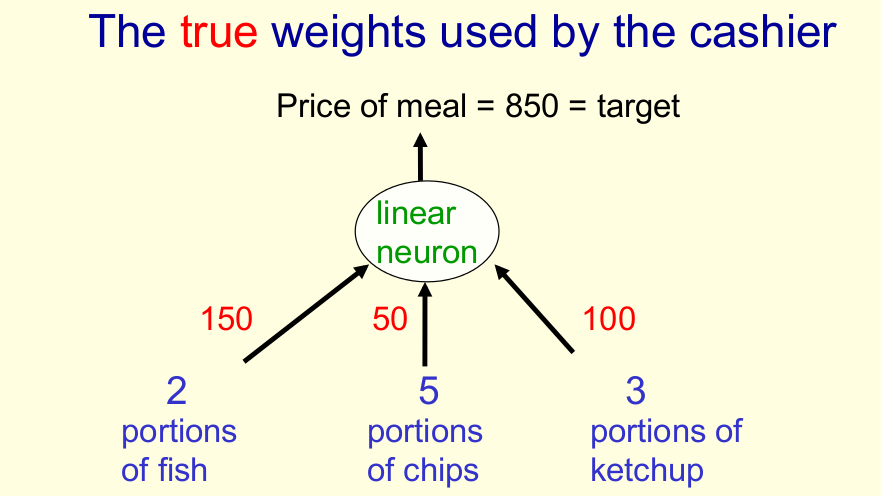
\includegraphics[width=3in]{/home/secondmath/Dropbox/GSPH/topic_review/DNN/mlpexam.png}
\caption{\bf {Example: Weight Estimation}}
\label{mlpexam}
\end{figure}


이 때 가격을 나타내는 vector $w$를 $w$=$(w_{fish},w_{chips},w_{ketchup})$과 같이 정의하고 error를 $\frac{1}{2}(t-y)^2$로 정의하면($y$: Estimation, $t$: Real), 우리의 목표는 에러값을 최소로 하는 $w$를 추정하는 것이 된다. 다층퍼셉트론에서는 모수$w_i$)들의 갯수가 너무 많아  회귀분석에서 쓰는 최소제곱추정량(Least Square Estimator), 최대가능도추정량(Maximum Likelihood Estimator)를 쓸 수 없고, 알고리즘을 이용하여 에러의 최소값에 가까워지게 해야 하는데 여기서 이용되는 것이 Gradient descent 방법이다. 이는 미분계수에 비례하여 모수를 수정한다는 것이 특징인데 이를 간단히 묘사하면 그림 \ref{gradient} 와 같다\cite{gradient}. 

\begin{figure}
\centering
\subfloat[Large Gradient]{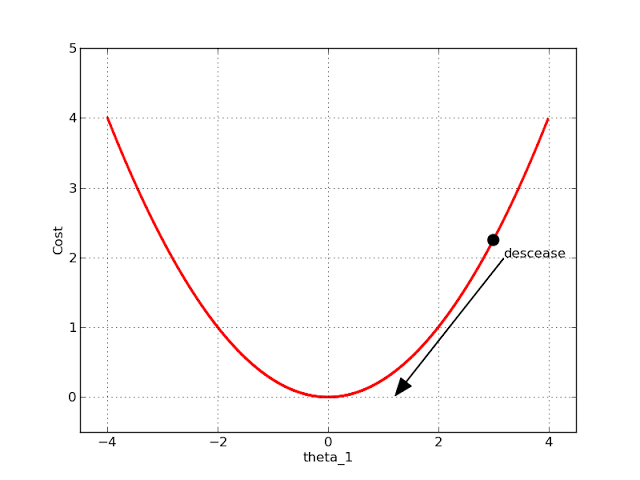
\includegraphics[width = 3in]{/home/secondmath/Dropbox/GSPH/topic_review/DNN/hy1.png}} 
\subfloat[Small Gradient]{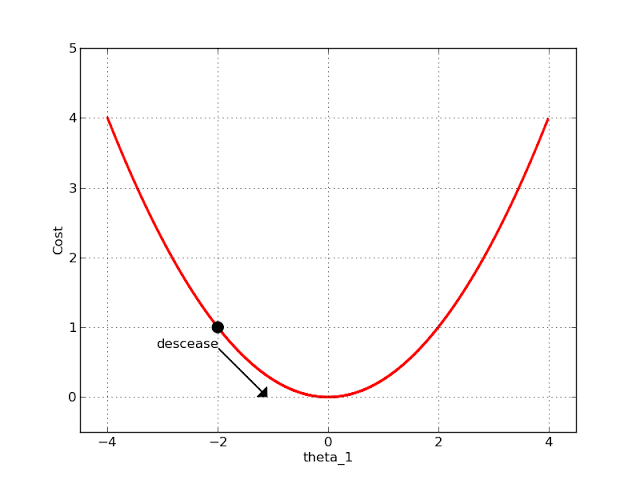
\includegraphics[width = 3in]{/home/secondmath/Dropbox/GSPH/topic_review/DNN/hy2.png}}\\
\subfloat[Small Learning Rate]{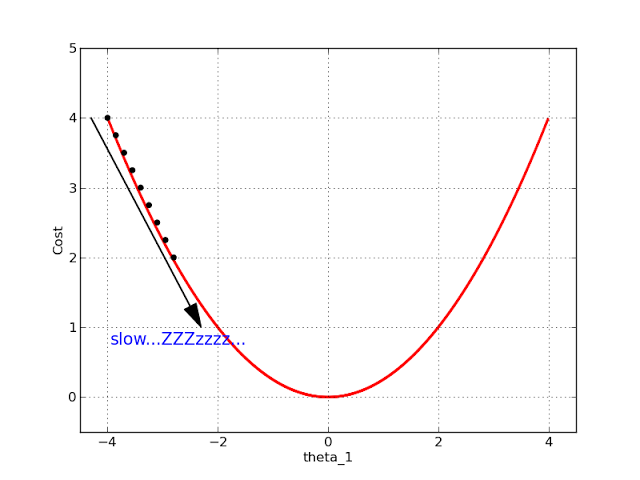
\includegraphics[width = 3in]{/home/secondmath/Dropbox/GSPH/topic_review/DNN/hy3.png}}
\subfloat[Large Learning Rate]{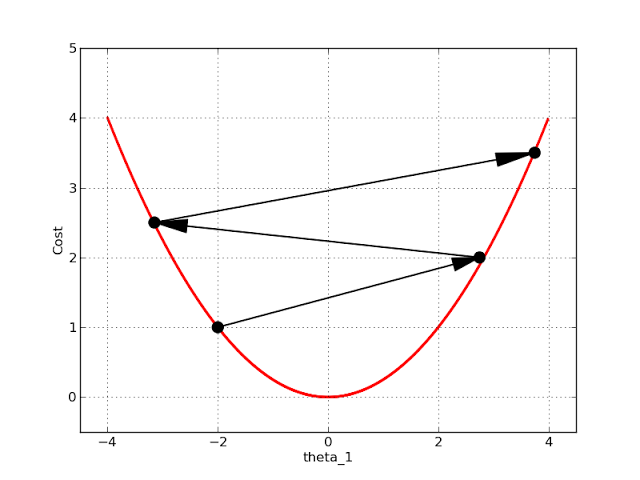
\includegraphics[width = 3in]{/home/secondmath/Dropbox/GSPH/topic_review/DNN/hy4.png}} 
\caption{\bf{Example: Gradient Descent Algorithm}}
\label{gradient}
\end{figure}

우리가 원하는 최소값일 때는 대부분 미분계수가 0일 때이므로 미분계수가 크면 크게 weight를 바꿔주고 미분계수가 작으면 작게 바꿔준다는 것이다. 또한 Learning rate를 결정할 수 있어서 얼마나 크게 바꿀지 대략적인 정도를 결정할 수도 있다. 

\begin{figure}[!ht]
\centering
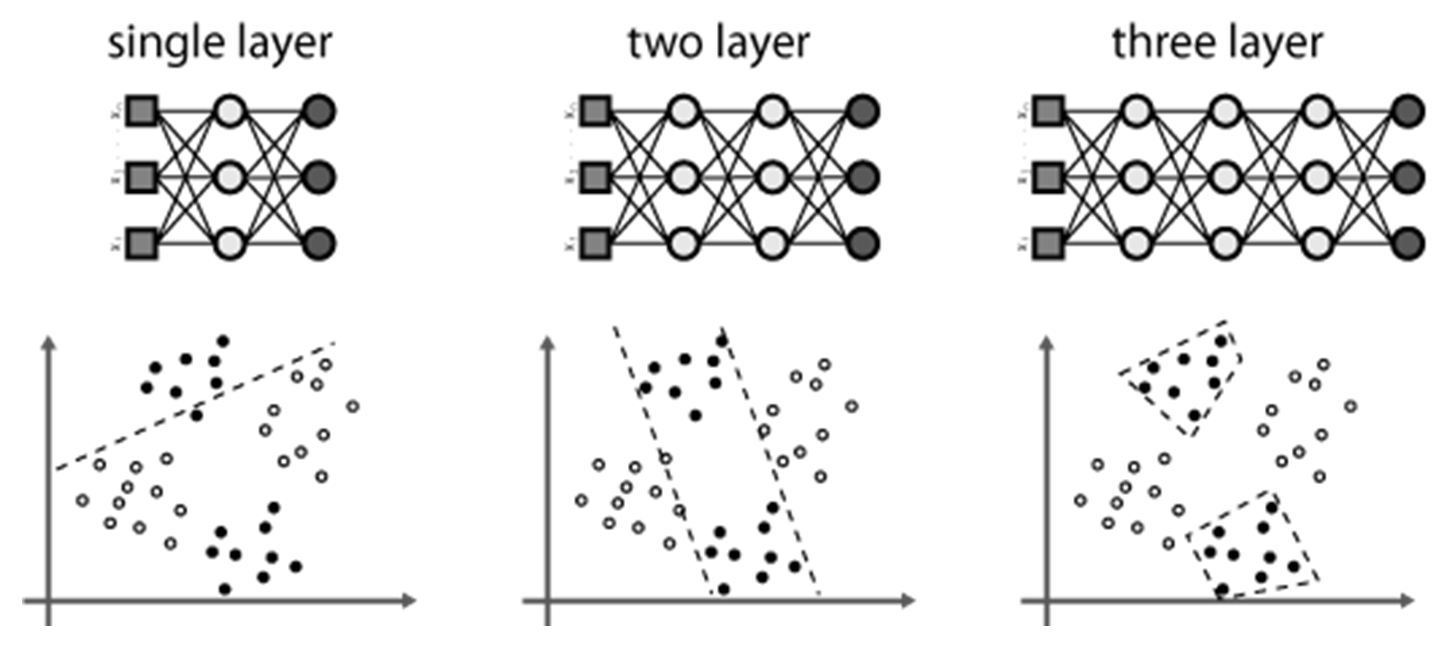
\includegraphics[width=5in]{/home/secondmath/Dropbox/GSPH/myreview/ml/neural3.jpg}
\caption{\bf{Multilayer Perceptron}}
\label{mlp}
\end{figure}


이제 이를 적용하여 예제를 풀어보자, 초기값으로 고기와 과자 케첩이 모두 50원이라고 하면 물고기 2개, 과자 5개, 케첩 3개의 전체 가격은 500원이 된다. 한편 에러함수를 각각 $w_i$에 대해 미분하면, 

\begin{align}
\frac{\partial E}{\partial w_i}= \frac{\partial y}{\partial w_i} \frac{dE}{dy}
\end{align}
가 되고 $E=\frac{1}{2}(t-y)^2$, $y=x_{fish}w_{fish} + x_{chips}w_{chips} + x_{ketchup}w_{ketchup}$을 대입하면 


\begin{align}
\frac{\partial E}{\partial w_i}= \frac{\partial y}{\partial w_i} \frac{dE}{dy}= - x_i(t-y)
\end{align}
가 되고 Learning rate를 감안한 $w_i$의 변화량은 
\begin{align}
\Delta w_i= -\epsilon \frac{\partial E}{\partial w_i}= \epsilon x_i(t-y)
\end{align}
이 된다. \\\\

대입해보면 $t$=850, $y$=500, $w_{fish}=w_{chips}=w_{ketchup}$=50 이고 간단한 계산을 위해 $\epsilon=\frac{1}{35}$로 하면 $\Delta w_{fish}$=20, $\Delta w_{chips}$=50, $\Delta w_{chips}$=30이 되고 이를 적용하면 다시 구해진 weight는 순서대로 70, 100, 80이 되며 이를 토대로 추정한 가격은 880이 된다. 이제 880과 850을 가지고 위의 과정을 계속 반복하면 참값에 가까운 값을 얻을 수 있을 것이다. \\\\

지금 설명한 것은 가장 기초적인 알고리즘을 설명한 것이며 실제 오류역전파 알고리즘은 초기 weight를 토대로 다층 hidden layer를 거쳐서 하나의 예측값을 구하고 그 예측값과 실제값의 차이를 토대로 역으로 weight들을 수정해 나가게 된다(그림 \ref{forback})\cite{kimjunmoppt}. 

\begin{figure}
\subfloat[Forward Propagation]{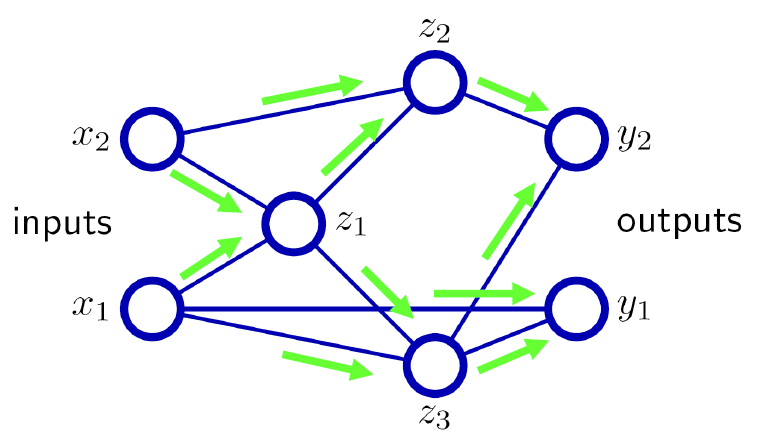
\includegraphics[width = 3in]{/home/secondmath/Dropbox/GSPH/topic_review/DNN/forward.png}} 
\subfloat[Back Propagation]{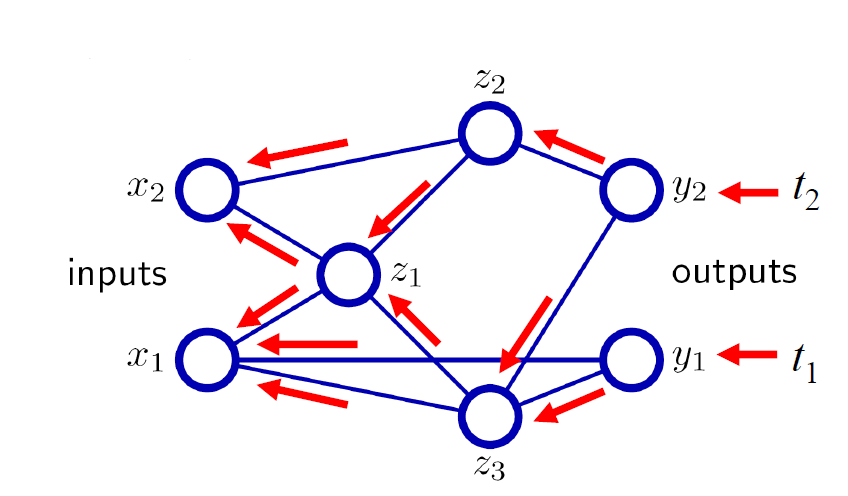
\includegraphics[width = 3in]{/home/secondmath/Dropbox/GSPH/topic_review/DNN/back.png}}
\caption{\bf{Backpropagation algorithm}}
\label{forback}
\end{figure}

에러역전파알고리즘으로 다층퍼셉트론을 학습할 수 있게 되었으나 이것을 실제로 사람들이 이용하기에는 많은 어려움이 따랐는데 그 이유들은 다음과 같다.
\begin{enumerate}
\item 수많은 Labeled data가 필요하다.
\item 학습을 하면 할수록 성능이 떨어진다(Vanishing gradient problem).
\item Overfitting problem 
\item Local minima에 빠질 가능성
\end{enumerate} 

하나씩 살펴보자. 추정해야 하는 모수가 많기 때문에 데이터가 많이 필요하고 그 중에서도 labeled data가 많이 필요하다. 허나 우리가 갖고 있는 데이터는 unlabeled data가 훨씬 많으며 실제 인간의 뇌의 학습 중 많은 부분이 unlabeled data를 이용한 Unsupervised Learning이며, 적은 양의 labeled data로 다층퍼셉트론을 학습하면 종종 hidden layer가 1개인 경우보다 성능이 떨어지는 경우를 관찰할 수 있으며 이것이 과적합(Overfitting)의 예시이다. \\

다음으로 Activation function을 살펴보면 logistic function이든 $tanh$ function이든 가운데 부분보다 양 끝이 현저히 기울기의 변화가 작은 것을 발견할 수 있다(그림 \ref{logistictan}). 때문에 학습이 진행될수록 급속도로 기울기아 0에 가까워져서 나중에는 거의 Gradient descent가 일어나지 않아 학습이 되지 않는 단점이 있다\cite{bengio1994learning}. 

\begin{figure}[!ht]
\centering
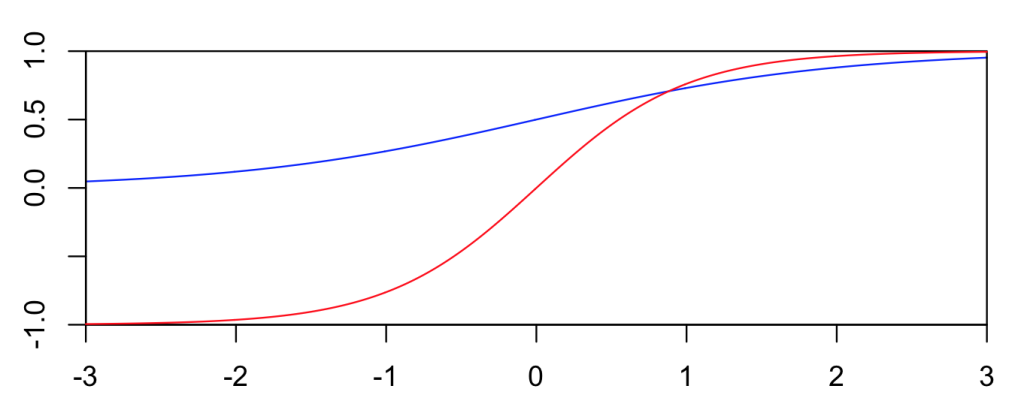
\includegraphics[width=5in]{/home/secondmath/Dropbox/GSPH/topic_review/DNN/logistictan.png}
\caption{\bf{Sigmoid functions}}
\label{logistictan}
\end{figure}



마지막으로 최소제곱추정량이나 최대가능도추정량등 직접적으로 최소값을 구하는 방법을 이용하지 못하고 알고리즘을 이용하여 최소값에 가까워지게 했기 때문에 학습에서 나온 최소값이 과연 진짜 최소값(Global minima)인가? 국소 최소값(Local minima)는 아닌가..에 대한 의문점이 풀리지 않게 된다. 시작점을 어떻게 두느냐에 따라 Local minima에 빠질 수도 있기 때문이다 (그림 \ref{minima})\cite{kimjunmoppt}. 이런 문제점들 때문에 실제로 Neural Network은 지지벡터머신(Support Vector Machine)등에 밀려 2000년 초까지 제대로 활용되지 못하였다.


\begin{figure}[!ht]
\centering
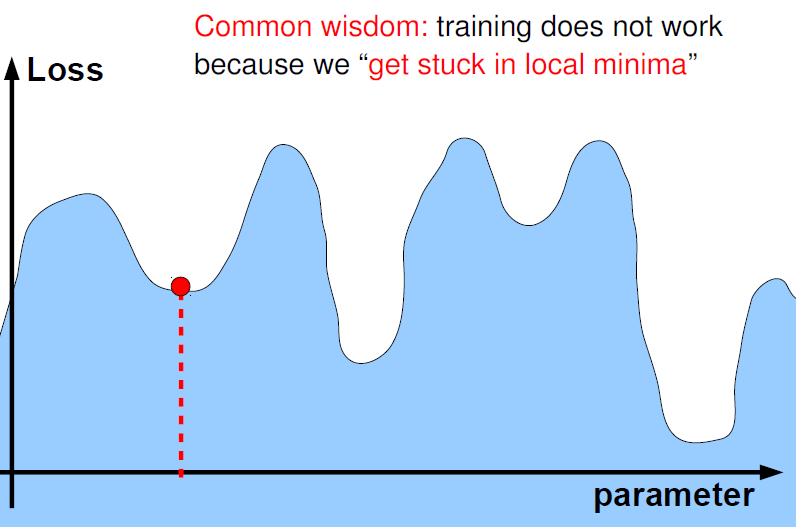
\includegraphics[width=4in]{/home/secondmath/Dropbox/GSPH/topic_review/DNN/minima.png}
\caption{\bf{Global and Local Minima}}
\label{minima}
\end{figure}

\subsection{3세대: Unsupervised Learning - Boltzmann Machine}
앞서 언급한 단점들 때문에 인공신경망 이론이 잘 이용되지 못하다가, 2006년 볼츠만 머신을 이용한 학습방법이 재조명되면서 인공신경망 이론이 다시 학계의 주목을 받게 되었는데 이 볼츠만 머신의 핵심 아이디어는 바로 Unsupervised Learning, 즉 label이 없는 데이터로 미리 충분한 학습을 한다는 것이며 그 후에 앞에 나온 역전파알고리즘 등을 통해 기존의 supervised learning을 수행한다\cite{smolensky1986information,hinton2006reducing}. 그림 \ref{unsupervised}에 대략적인 묘사가 표현되어 있는데 아기들은 단어나 음, 문장의 뜻을 전혀 모르는 상태로 학습을 시작하게 되고 음소(phoneme),  단어(word), 문장(sentence)순으로 Unsupervised learning을 수행하게 되며 그 후에 정답을 가지고 supervised learning을 수행하게 된다\cite{kimjunmoppt}. 이런 방법을 통해 앞서 언급한 다중 퍼셉트론의 단점들이 많이 해결되는데, Unlabeled data를 이용할 수 있고 이를 이용해 unsupervised pre-training을 수행함으로서 vanishing gradient problem, overfitting problem이 극복될 수 있으며, pre-training이 올바른 초기값 선정에도 도움을 주어 local minima problem도 해결할 수 있을 것이라 여겨지고 있다\cite{bengio2009learning}. 이에 본 글에서는 가장 대표적인 방법인 Deep Belief Network(DBN)과 이를 수행하기 위해 필요한 Restrict Boltzmann Machine(RBM)에 대하여 간단히 설명하기로 하겠다. 

\begin{figure}[!ht]
\centering
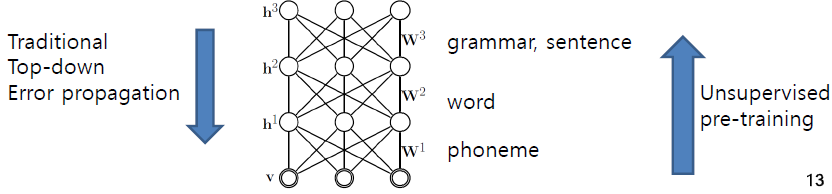
\includegraphics[width=5in]{/home/secondmath/Dropbox/GSPH/topic_review/DNN/unsupervised.png}
\caption{\bf{Description of Unsupervised Learning}}
\label{unsupervised}
\end{figure}

\paragraph{Restricted Boltzmann Machine(RBM)}
볼츠만 머신은 visible layer와 1개의 hidden layer로 이루어진 방향이 없는 그래프(undirected graph)로 이루어져 있다. 이것의 특징은 Energy based model이라는 점인데 Energy based model이라는 것은 어떤 상태가 나올 확률밀도 함수를 에너지의 형태로 나타내겠다는 것이며  visible unit의 벡터를 $v$, hidden unit의 벡터를 $h$라 하면($v$,$h$: binary vector- 0 or 1) 볼츠만 머신의 그래프와 확률밀도함수는 다음과 같다(그림 \ref{RBM})\cite{lecun2006tutorial,lecun2005loss}.

\begin{figure}[!ht]
\centering
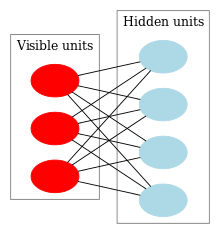
\includegraphics[width=3in]{/home/secondmath/Dropbox/GSPH/topic_review/DNN/RBM.png}
\caption{\bf{Diagram of a Restricted Boltzmann\cite{RBMfigure}}}
\label{RBM}
\end{figure}


\begin{align}\label{pdf}
P(v,h)=\frac{1}{Z}\exp^{-E(v,h)}
\end{align}
(Z: Normalized Constant)\\

그림 \ref{RBM}을 보면 $v$끼리는 선이 연결되어 있지 않고 $h$끼리도 마찬가지인데 이것이 Restricted의 의미이며 이 조건이 없으면 그냥 Boltmann Machine이며 RBM형태의 그래프를 이분그래프(bipartite graph)라 한다. 그냥 Boltzmann Machine은 너무 복잡해서 학습이 어려워 그 대안으로 나온 것이 RBM인 것이다. 한편 식 \ref{pdf}를 보면 그래프의 에너지 상태가 낮을수록 확률이 작아지는 것을 알 수 있는데 이 가정은 물리학의 열역학 2법칙을 연상시킨다. 이제 RBM의 Energy function을 살펴보면 

\begin{align}\label{energy}
E(v,h)= -\sum_i a_i v_i - \sum_j b_j h_j -\sum_i \sum_j h_j w_{i,j} v_i=-a^{\mathrm{T}} v - b^{\mathrm{T}} h -h^{\mathrm{T}} W v
\end{align}
($a_i$: offset of visible variable, $b_j$: offset of hidden variable, $w_{i,j}$: weight between $v_i$ and $h_j$)\\
에너지에 대한 수식에서 눈여겨 보아야 할 부분이 $\sum_j h_j w_{i,j} v_i$인데, $v_i$, $h_j$가 1인 곳에 weight가 클수록 에너지함수 값이 작아지고 결과적으로 확률밀도함수의 값이 높아진다. 이는 인간의 시냅스에서 일어나는 일과 비슷한데, 같이 켜지는 곳이 시냅스로 연결될 가능성이 높기 때문이다(그림 \ref{Hebb}).

\begin{figure}[!ht]
\centering
\subfloat{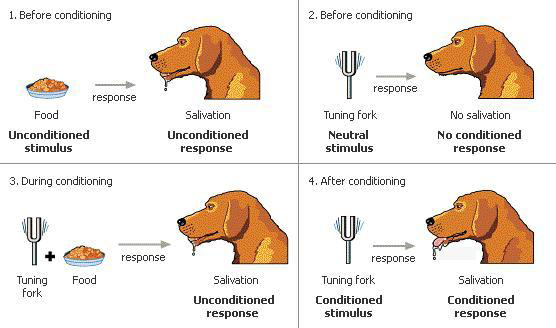
\includegraphics[width = 3.2in]{/home/secondmath/Dropbox/GSPH/topic_review/DNN/dog.png}} 
\subfloat{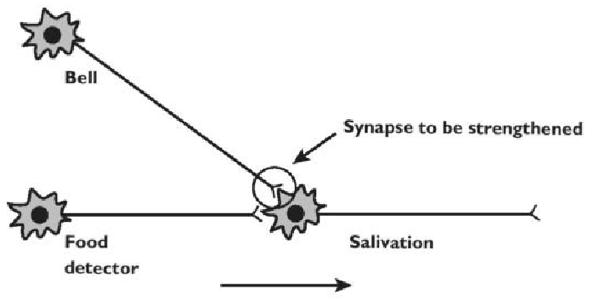
\includegraphics[width = 3.2in]{/home/secondmath/Dropbox/GSPH/topic_review/DNN/dog2.png}}
\caption{\bf{Hebb's Law}\cite{hebb2,kimjunmoppt}}
\label{Hebb}
\end{figure}


이제 우리가 원하는 것은 $P(v)=\sum_h P(v,h)$ 의 최댓값을 구하는 것인데 RBM은 이분그래프로 v끼리, h끼리는 전부 독립이므로 
\begin{subequations}
 \label{RBMcondition}
 \begin{align}
  P(v|h) = \prod_{i=1}^m P(v_i|h) \label{eq11} \\
  P(h|v) = \prod_{j=1}^n P(h_j|v) \label{eq12}
 \end{align}
\end{subequations}


로 간단히 분리할 수 있으며, 이에 따른 individual activation probabilities는 
\begin{subequations}
 \label{RBMindi}
 \begin{align}
  p(h_j=1|v) = \sigma \left(b_j + \sum_{i=1}^m w_{i,j} v_i \right) \label{eq13} \\
  p(v_i=1|h) = \sigma \left(a_i + \sum_{j=1}^n w_{i,j} h_j \right) \label{eq14}
 \end{align}
\end{subequations}
로 표현할 수 있다($\sigma$: activation function). 이 장점을 이용하여 Gibbs sampling을 쓰면서 weight를 수정해 나가면  간단히 $logP(v)$의 최댓값과 그때의 weight들을 구할 수 있는데 이 방법에 대해 간략히 알아보겠다. 

\paragraph{Training RBM}
기본적인 아이디어는 앞서 퍼셉트론에서 언급한 Gradient descent 방법과 일치한다. 기울기(미분계수)에 비례해서 감소시키면 결국 minima에 도달할 것이라는 아이디어인데 RBM에서는 $logP(v)$의 최댓값과 그때의 $w$, $a$ , $b$ 들을 구하는 것이 목적이므로 Gradient descent의 반대 방향으로 알고리즘을 쓰면 된다(Gradient ascent). 한편 $logP(v)$를 다시 표현하면 

\begin{align}
logP(v)=log(\sum_{h} \frac{\exp^{-E(v,h)}}{Z})=log(\sum_h \exp^{-E(v,h)})-logZ=log(\sum_h \exp^{-E(v,h)})-log(\sum_{v,h} \exp^{-E(v,h)})
\end{align}

과 같고 이를 미분하면 


\begin{subequations}
 \label{RBMdiff}
 \begin{align}
  \frac{\partial logP(v)}{\partial \theta}&=-\frac{1}{\sum_h \exp^{-E(v,h)}} \sum_h \exp^{-E(v,h)}\frac{\partial E(v,h)}{\partial \theta}+\frac{1}{\sum_{v,h} \exp^{-E(v,h)}} \sum_{v,h} \exp^{-E(v,h)}\frac{\partial E(v,h)}{\partial \theta} \\
  &= -\sum_{h} p(h\mid v) \frac{\partial E(v,h)}{\partial \theta} + \sum_{v,h} p(h,v)\frac{\partial E(v,h)}{\partial \theta} \label{kkk}
 \end{align}
\end{subequations}

과 같고 여기서 식 \ref{kkk}를 살펴보면 first term은 $\frac{\partial E(v,h)}{\partial \theta}$를 $p(h|v)$를 가지고 평균을 낸 것이고, second term은 같은 것을 $p(h,v)$의 확률분포를 기반으로 평균을 낸 것이라 할 수 있다. 이 들은 모두 Gibbs sampling을 이용하여 sampling할 수 있는데 여기서는 일반적인 Gibbs sampling과는 약간 다른 Contrastive Divergence(CD-$k$) 방법을 쓰게 된다. CD-$k$의 과정을 간단히 설명하면 처음엔 training sample에서 $v$를 random sampling하고 그 $v$를 대상으로 $p(h|v)$ 함수를 이용하여 first term을 해결하며, 그 다음으로는 계속 이어서 $k$-1번의 횟수동안 $p(h|v)$, $p(v|h)$ 함수를 이용하여 sampling을 수행하여 나온 $v^{(k)}$를 이용하여 second term을 해결한다는 것이다. $k$는 보통 1으로도 충분하다고 알려져 있으며 위의 과정을 를 수행하여 나온 값을 기반으로 $w$, $a$, $b$를 업데이트 하고 같은 과정을 반복해나가면 되는 것이다. 이를 pseudocode로 요약하면 그림 \ref{cdk}와 같다. 

\begin{figure}[!ht]
\centering
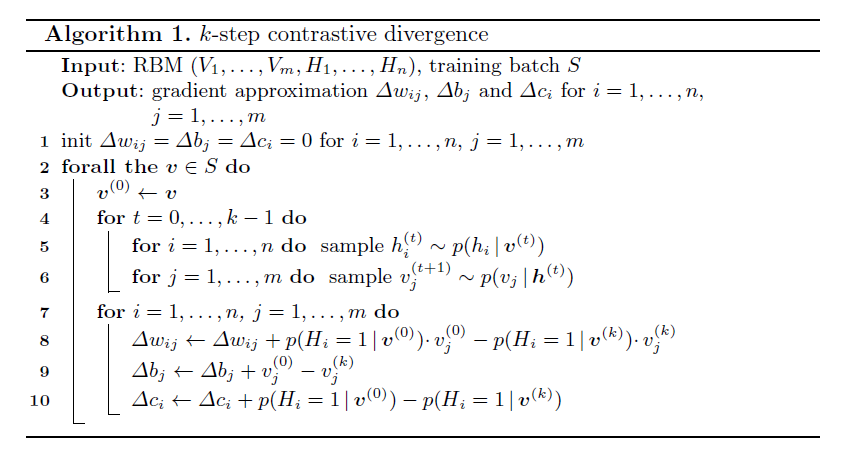
\includegraphics[width=5in]{/home/secondmath/Dropbox/GSPH/topic_review/DNN/cdk.png}
\caption{\bf{Contrastive Divergence(CD-$k$)\cite{fischer2012introduction}}}
\label{cdk}
\end{figure}


\paragraph{Deep Belief Network(DBN)}
DBN은 간략히 말하면 RBM을 여러 층으로 쌓은 것인데 그림 \ref{dbn}에 대략적인 묘사가 되어 있다. 즉 RBM을 여러 층을 두어 학습하고 마지막으로 기존의 오류역전파알고리즘을 이용하여 튜닝(Fine tuning)하는 것이다\cite{hinton2006fast,hinton2009deep,bengio2009learning}. 이는 위에 예시로 든 아기가 언어를 학습하는 방식인 음소(phoneme),  단어(word), 문장(sentence)순의 Unsupervised training과 그 후의 supervised learning을 반영하는 모형이라 할 수 있다. 

\begin{figure}[!ht]
\centering
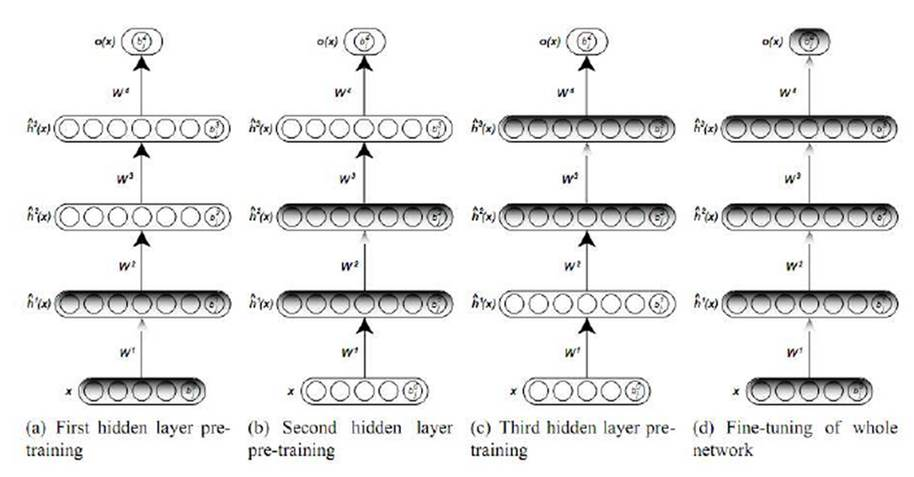
\includegraphics[width=5.5in]{/home/secondmath/Dropbox/GSPH/topic_review/DNN/dbn.jpg}
\caption{\bf{Deep Belief Network\cite{dbnfig}}}
\label{dbn}
\end{figure}

DBN은 각각의 과정에서 확률적으로 hidden layer들의 값을 생성하게 되는데 이를 역으로 진행하면 정답을 토대로 input을 생성할 수도 있다. 이를 generative model이라 하는데 Hinton교수의 홈페이지 \url{http://www.cs.toronto.edu/~hinton/adi/index.htm}에 손으로 쓴 숫자인식에 대한 예제가 나와 있으니 참고하기 바란다. 

\paragraph{기타}
이외에도 locally connected convolution layer를 이용한 Convolutional RBM, 텍스트와 이미지를 동시에 학습할 수 있는 Multimodal Learning에 유용한 Deep Boltzmann Machine(DBM) 등이 있는데 이것들은 참고문헌을 참고하길 바란다\cite{lee2009convolutional,salakhutdinov2009deep}. 

\subsection{3세대: Supervised Learning - Rectified linear unit (ReLU), Dropout} 
RBM을 이용한 Unsupervised learning을 이용하게 되면서 다층퍼셉트론의 약점이 많은 부분 극복되었다. Unlabeled data를 사용할 수 있게 되었고 이를 충분히 활용하여 overfitting issue, vanishing gradient문제가 해결되었고 pre-training이 좋은 시작점을 제공하여 local minima 문제도 해결되는 것처럼 보였다. 한편, 언급된 다층퍼셉트론의 약점을 그냥 Supervised Learning에서 해법을 찾으려는 최근의 노력들이 있었고 그 결과로 지금까지 나온 대표적인 아이디어가 Rectified linear unit(ReLU), Dropout이다. 본 섹션에서는 이 두 방법에 대해 간단히 소개하도록 하겠다. 

\paragraph{Rectified linear unit (ReLU)}
Vanishing gradient 즉, 학습을 할수록 weight의 기울기가 0에 급속도로 가까워 지는 것이 다층퍼셉트론(multilayer perceptron)에서 학습이 어려운 이유 중 하나였다. 이는 activation함수의 모양에서 기인하는데 그림 \ref{logistictan}을 다시 살펴보면 logistic function이든 $tanh$함수이든 가운데 부분만 기울기가 가파르고 양끝으로 갈수록 기울기가 급속도로 0에 가까워지는 것을 볼 수 있고 이것이 vanishing gradient의 실제이다. 2010년과 2011년에 걸쳐 이를 극복하기 위한 아이디어가 제시되었는데 그것이 바로 Rectified linear unit(ReLU)이다. 이름에서 직관적으로 느낄 수 있듯이 이는 $x$가 0이상일 때는 선형증가하는 함수이며 0미만일 때는 모두 0인 함수인데, 그림 \ref{relu}에서 볼 수 있듯이 0보다만 크면 항상 기울기가 1로 일정해 기울기가 감소하는 경우가 없어 학습이 용이하며 실제로 이것이 기존의 방법보다 학습성능이 좋고 pre-training의 필요성을 없애준다고 알려져 있다\cite{nair2010rectified,glorot2011deep}. 


\begin{figure}[!ht]
\centering
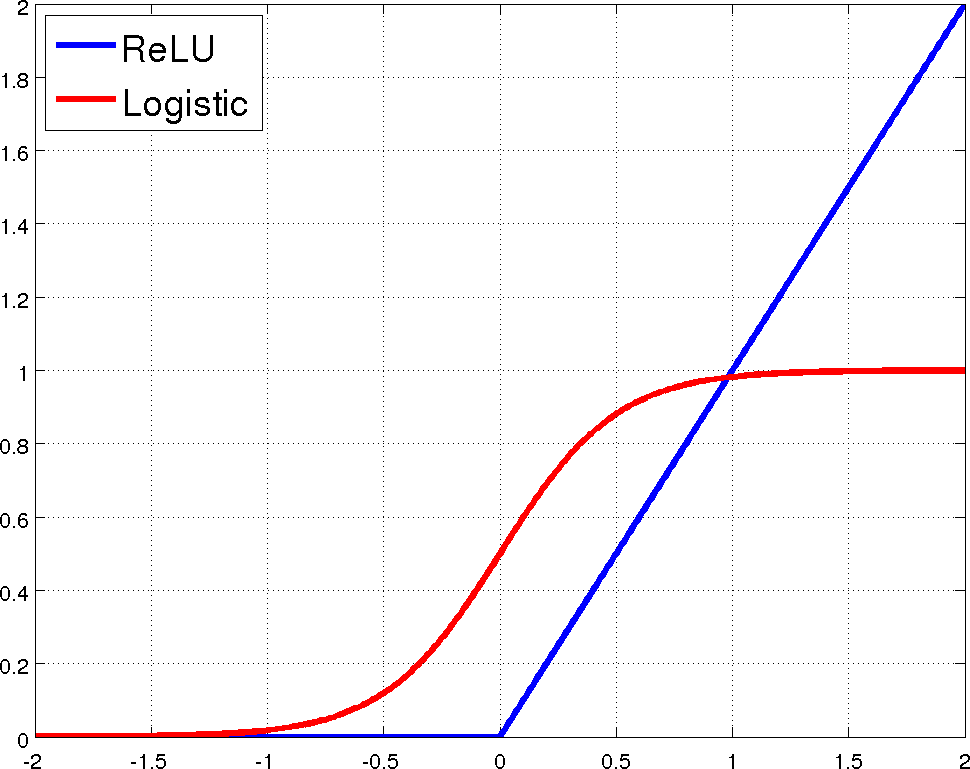
\includegraphics[width=3in]{/home/secondmath/Dropbox/GSPH/topic_review/DNN/relu.png}
\caption{\bf{The proposed non-linearity, ReLU, and the standard neural network non-linearity, logistic\cite{zeiler2013rectified}}}
\label{relu}
\end{figure}


\paragraph{DropOut}
Labeled data의 부족 및 그로 인한 overfitting 즉, hidden layer들은 많은데 labeled data의 수가 적은 것도 다층퍼셉트론 학습이 어려운 이유 중 하나였다. 이에 Hinton교수는 2012년에 \textbf{DropOut}이라는 방법을 제안하는데 이는 기본적으로 여러개의 모형을 합쳐서 새로운 모형을 만드는 Ensemble 모형과 유사하다\cite{hinton2012improving}. Training example을 학습할 때 마다 모든 hidden unit을 50\%의 확률로 끄는(DropOut)것인데 이를 비유하자면 회사에서 모든 팀이 모든 일을 함께 하는 것보다 팀별로 분담해서 일을 한 후 그것을 통합하는 것이 더 효율적으로 업무를 수행할 수 있는 것과 비슷하다고 할 수 있다. 즉, 각 데이터를 학습할 때마다 hidden unit의 절반만 써서 결론적으로 그 학습결과를 합치면 기존의 학습방법보다 좋은 성능을 보인다는 것이다. 2013년에는 이 아이디어를 확장하여 DropConnect라는 방법이 제안되었는데, 이것은 hidden unit을 끄는 대신 hidden unit과의 연결을 50\%의 확률로 꺼서 학습하는 점이 DropOut과의 차이점이다(그림 \ref{dropfig1})\cite{wan2013regularization}. 

\begin{figure}[!ht]
\centering
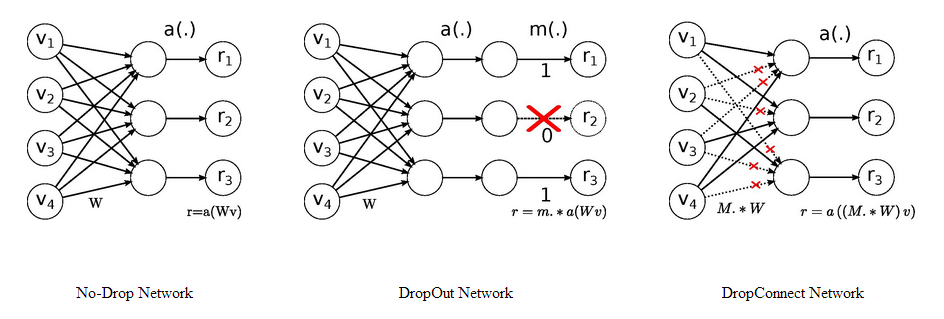
\includegraphics[width=6in]{/home/secondmath/Dropbox/GSPH/topic_review/DNN/dropout.png}
\caption{\bf{Description of DropOut \& DropConnect\cite{dropfig}}}
\label{dropfig1}
\end{figure}

그림 \ref{dropperformance}에 나와있듯이 실제로 DropOut과 DropConnect의 성능이 그렇지 않은 경우보다 우수함이 알려져 있다\cite{wan2013regularization}.

\begin{figure}[!ht]
\centering
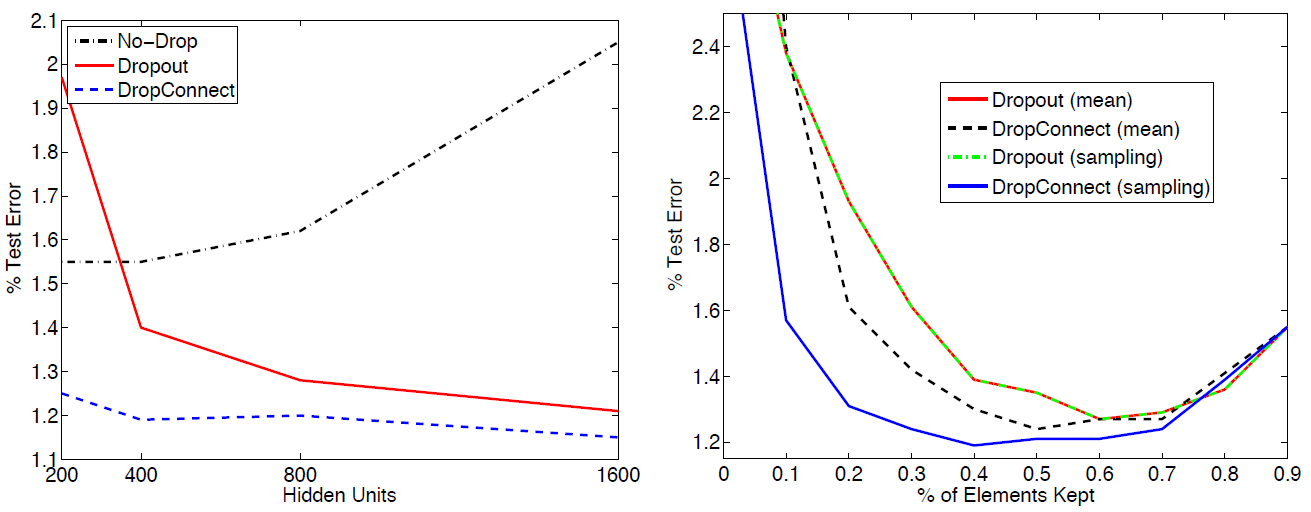
\includegraphics[width=6in]{/home/secondmath/Dropbox/GSPH/topic_review/DNN/dropperformance.png}
\caption{\bf{Using the MNIST dataset, in a) Ability of Dropout and DropConnect to prevent overfitting as the size of the 2 fully connected layers increase. b) Varying the drop-rate in a 400-400 network shows near optimal performance around the $p$ = 0.5\cite{wan2013regularization}}}
\label{dropperformance}
\end{figure}

\paragraph{Local minima issue}
우리가 구한 에러의 최소값이 실제 Global minima인가.. local minima에 빠지는 것은 아닌가.. 라는 문제도 오랫동안 다층퍼셉트론에서의 이슈였는데 현재의 공감대는 High dimension and non-convex optimization에서는 대부분의 local minima들의 값이 비슷비슷할 것이며 따라서 local minima나 global minima나 크게 차이가 없을 것이고 너무 이 문제에 신경쓸 필요가 없다는 점이다(그림 \ref{localminima})\cite{minima}. 수많은 차원에서 차원마다 local minima이기는 쉽지 않다고 직관적으로 이해할 수 있다.  

\begin{figure}[!ht]
\centering
\includegraphics[width=4in,page=31]{/home/secondmath/Dropbox/GSPH/topic_review/DNN/ranzato.pdf}
\caption{\bf{Local minima when high dimension and non-convex optimization \cite{minima}}}
\label{localminima}
\end{figure}


\section{딥러닝 요약}
1950년대 퍼셉트론(perceptron)에서 시작된 인공신경망 연구는 1980년대 오류역전파알고리즘(Error Backpropagation Algorithm)으로 다층퍼셉트론(Multilayer perceptron)을 학습할 수 있게 되면서 발전을 이루었다. 허나 Gradient vanishing, labeled data의 부족, overfitting, local minima issue 등이 잘 해결되지 못해 2000년대 초까지 인공신경망 연구는 답보를 이루고 있는데, 2006년부터 볼츠만머신을 이용한 Unsupervised Learning인 Restricted Boltzmann Machine(RBM), Deep Belief Network(DBN), Deep Boltzmann Machine(DBM), Convolutional Deep Belief Network 등이 개발되면서 unlabeled data를 이용하여 pre-training을 수행할 수 있게 되어 위에 언급된 다층퍼셉트론의 한계점이 극복되었다. 2010년부터는 빅데이터를 적극적으로 이용함으로서 수많은 labeled data를 사용할 수 있게 되었고, Rectified linear unit (ReLU), DropOut, DropConnect 등의 발견으로 vanishing gradient문제와 overfitting issue를 해결하여 아예 Supervised learning이 가능하게 되었으며, local minima issue도 High dimension non-convex optimization에서는 별로 중요한 부분이 아니라는 공감대가 확장되고 있다. 


\section{고찰: 보건학으로의 적용}
딥러닝의 특징은 크게 기계학습으로서의 특징과 다른 기계학습방법과 구별되는 딥러닝만의 특징으로 나눌 수 있는데 본문에서는 이를 보건학에서의 역학연구와 같이 비교해 보겠다.


\paragraph{역학 vs 기계학습}
통계학자 칼 피어슨은 진화론의 증명을 위해 통계학을 이용하였으며, R.A Fisher는 가장 성능이 좋은 비료를 선택하기 위해 통계학을 이용하였는데 전자는 지식의 확장으로 역학연구에서 이용하는 통계학에 해당하며, 후자는 올바른 의사결정을 위한 것으로 기계학습에서 사용하는 통계학이라고 볼 수 있다. 즉, 역학은 기본적으로 인과관계 해석(causal inference)가 목적인데 반해, 기계학습은 예측(prediction)이 주 목적이라는 것이다. 목적의 차이는 모형선택의 차이로 이어지게 되는데, 역학연구에서는 인과관계의 증명, 결과의 해석이 중요하기 때문에 모형선택도 이것을 잘 할 수 있는 것이 최우선 기준이다. 즉, 해석이 간단한 모형(선형회귀 or 로지스틱회귀분석이 Odds Ratio)이 선호되며 결과가 진짜 믿을만한 결과인지 아닌지가 중요하게 되어 $P-value$, $\beta$, Odds Ratio(OR), Hazard Ratio(HR), 내적 타당도 등이 중요한 지표가 된다. 반면 기계학습에서는 얼마나 잘 예측하는지가 중요하기 때문에 복잡한 모형을 선택하는 것을 주저하지 않으며 인간이 해석하기 어려운 모형도 예측력만 좋다면 적용할 수 있다. 또한 $\beta$나 $p-value$ 등의 해석을 위한 지표보다는 $\hat{y}$,$\hat{p}$, cross-validation, ROC curve, AUC(Area Under Curve), 외적 타당도 등의 예측을 나타내는 지표들이 중요한 지표가 된다. 


\paragraph{딥러닝 vs 다른 기계학습}
딥러닝은 뇌의 작용을 모형화 한 것으로 다수의 hidden layer들을 토대로 병렬연산을 수행하는 방법으로 기계학습 중에서도 모형의 flexibility가 가장 큰 편에 속하여 모형을 인간이 이해하기가 어려운데, 이는 우리가 뇌의 메커니즘에 대해 모르는 부분이 많은 것과 일맥상통하다고 할 수 있다. 이 중에서도 대량의 \textbf{병렬연산(parallel computing)}이야 말로 딥러닝의 특징적인 부분이며 최근 Google 등의 글로벌 IT회사에서 하는 패턴인식연구를 살펴보면 GPU(Graphical Processor Unit)를 사용하여 수천에서 수만개의 Core를 사용한 병렬연산을 수행하는 것을 알 수 있다\cite{le2013building,coates2013deep}. 병렬연산을 위한 프로그래밍언어인 CUDA(Compute Unified Device Architecture), OpenCL 등도 개발되어 병렬컴퓨팅에 이용되고 있으며 앞으로 이 언어들의 중요성이 더 커질 것이라 생각한다\cite{nvidia2007compute,stone2010opencl}.

\paragraph{가설검정(hypothesis testing) vs 가설생성(hypothesis generating)}
앞서 언급한 역학연구와 기계학습의 차이점에 덧붙여 빅데이터(Big Data)를 이용할 수 있게 되고 컴퓨터의 성능이 이를 뒷받침하면서 과학연구의 패러다임도 바뀌고 있는데 가설생성이 바로 그것이다\cite{biesecker2013hypothesis}. 기존의 과학연구가 선행연구를 통해 가설을 설정하고 그에 맞게 데이터를 모아 가설을 검정하고 지식을 확장하였다면, 가설생성은 철저히 데이터를 올바르게 해석하는 것에 중점을 둔 것이다. 빅데이터를 토대로 그것의 패턴을 면밀히 분석하면 새로운 가설을 설정할 수 있고 이를 검정하여 지식을 확장하면 되는 것이다(그림 \ref{hypogenerate}). 

\begin{figure}[!ht]
\centering
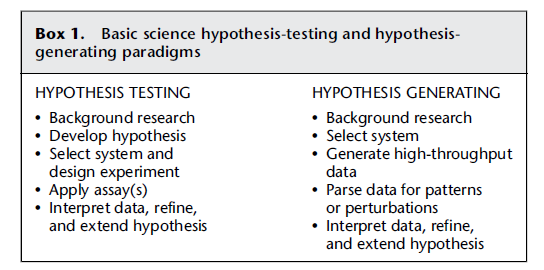
\includegraphics[width=4in]{/home/secondmath/Dropbox/GSPH/topic_review/DNN/textmining7.png}
\caption{\bf{Basic science hypothesis-testing and hypothesisgenerating
paradigms \cite{biesecker2013hypothesis}}}
\label{hypogenerate}
\end{figure}


지금까지 딥러닝의 개념, 역사와 현재, 그리고 기존의 역학연구와의 차이점에 대해 알아보았다. 모바일 기기를 이용한 보건학에서 가장 중요한 것은 모바일 기기를 통해 생성되는 빅데이터를 효과적으로 분석하는 것이며 그 데이터는 대부분 영상, 음성, 텍스트가 될 것임이 자명하다. 따라서 이런 비정형 빅데이터를 효과적으로 분석할 수 있는 딥러닝이 Mobile Health의 핵심 기술이 될 것임은 의심할 여지가 없을 것이며, 이 기술을 보건학에서도 적극적으로 활용해야 한다. 이를 위해 최신 병렬 프로그래밍 언어의 활용과 슈퍼컴퓨터 시설의 구축에도 힘써야 할 것이며, 꼭 딥러닝이 아니더라도 전반적인 기계학습과 가설생성의 철학에 대한 이해가 반드시 필요하며 기존의 역학연구의 causal inference의 패러다임에서 벗어나 빅데이터와 예측모형이라는 새로운 패러다임에 적응해야 할 것이다. 


\bibliographystyle{abbrv}
\bibliography{DNN}

\end{document}
